\documentclass{jsarticle}
\usepackage[dvipdfmx]{graphicx}
\begin{document}

\title{数値計算レポート}
\author{IS5 14 佐々木 結大}
\maketitle
\newpage
\tableofcontents
\newpage

\section{本レポートについて}
本レポートは、ラグランジュ補間と最小二乗法について調査と実装を行い、
その特徴を考察して報告するものである。
\section{ラグランジュ補間}
\subsection{補間}
補間とは、いくつかの既に分かっている値から、その間の数値を求めることである。
ラグランジュ補間は、いくつかの2次元の点を与えられ、それらを全て通るグラフを求めることで、
2次元の点の間を結ぶ線を求め、それによって与えられた点の間にある点を求めることができる。
\subsection{実験方法}
以下の4つの点を通る関数を、ラグランジュ補間によって求める。
\[
    (-1.0,2.0),
    (0.0,5.0),
    (2.0,-1.0),
    (3.0,2.0)
\] 
これら4つの点を通る関数は、
\[
    y=x^3-3x^2-x+5
\]
である。
ラグランジュ補間によって\(x\)が\([-1.0,3.0]\)の
範囲で0.1刻みで計算し、正しく関数が求められているかを確認する。
また、前述の4点を正しく通っているか調べる。
図\ref{fig:lag_ingraph} の赤い線が補間する関数
\(y=x^3-3x^2-x+5\)であり、オレンジの点が入力として与えた点である。

\begin{figure}[htbp]
    \begin{center}
    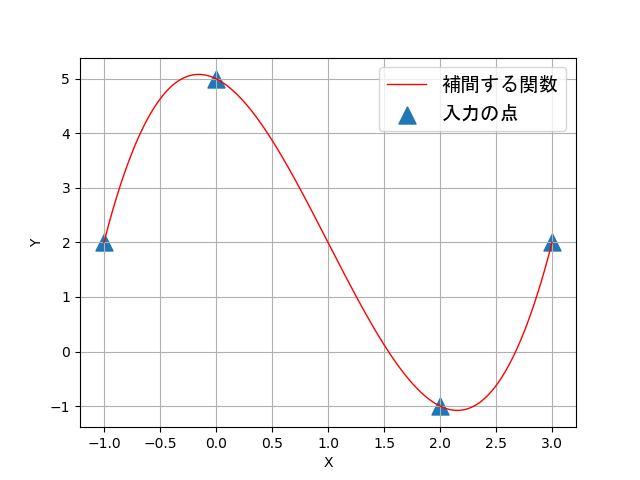
\includegraphics[width=0.5\hsize]{lag_in.png}
    \caption{入力する点列}\label{fig:lag_ingraph} 
    \end{center}
\end{figure}

\subsection{ラグランジュ補間}
ラグランジュ補間では、以下の\(x\)の関数を使用する。
\begin{equation}
    f(x)=\sum^n_{k=0}y_k\frac{f_k(x)}{f_k(x_k)}
    \label{eq:lageq} 
\end{equation}

ここで、\(n\)は入力として与えられる点の数、
\((x_k,y_k)\)は、その座標である。
\(f_k\)は、以下のものである。
\begin{equation}
    f_k(x)=(x-x_0)(x-x_1)\cdots (x-x_{k-1})(x-x_{k+1})\cdots (x-x_{n-1})
    \label{eq:legeq2}
\end{equation}

この式に従って計算を行えば、すべての実数\(x\)での値を補間することができると考えられる。
式\ref{eq:lageq}の和の内側は、\(x\)のn-1次関数である。

(\(y_k\)は実数、\(f_k(x_k)\)も実数に関数を適応した実数であることに注意。)

この和である式\ref{eq:lageq}もまたn-1次関数となる。

ここで、\ref{eq:lageq}のn次関数\(f(x)\)が、与えられたすべての点
\(x_i,y_i\)を通ることを示す。
\(f(x)\)にある\(x_i,y_i\)を代入すると、
\begin{eqnarray*}
    f(x_i)& = & \sum^n_{k=0}y_k\frac{f_k(x_i)}{f_k(x_k)} \\
    & = & y_k\frac{
        (x_i-x_0)(x_i-x_1)\cdots (x_i-x_{i-1})(x_i-x_{i+1})\cdots (x_i-x_{n-1})
    }{
        (x_i-x_0)(x_i-x_1)\cdots (x_i-x_{i-1})(x_i-x_{i+1})\cdots (x_i-x_{n-1})
    } \\
    & = & y_k 
\end{eqnarray*}
となる。(\(i=k\)以外の項は0になる。)
\subsection{結果と考察}
結果を図\ref{fig:laggraph} に示す。赤い線が補間する関数
\(y=x^3-3x^2-x+5\)であり、青い点がラグランジュ補間で
計算した値、オレンジの点が入力として与えた点である。

\begin{figure}[htbp]
    \begin{center}
        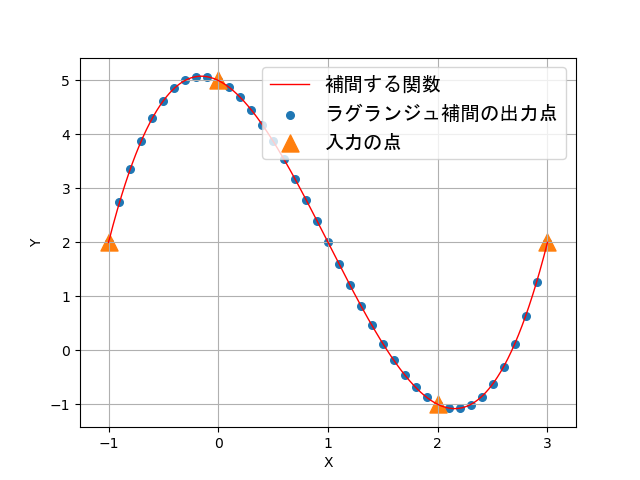
\includegraphics[width=0.5\hsize]{lag.png}
        \caption{ラグランジュ補間}\label{fig:laggraph}      
    \end{center}
\end{figure}
与えられたオレンジの点を通る関数を求め、それを使って入力の点の間の点を
補間していることがわかる。



\section{最小二乗法}
\subsection{近似}
多くの点が与えられ、そのすべてを通る関数を求めることができない場合に、
なるべくすべての点との差が小さくなるような関数を求めることを考える。
これを関数によって近似するという。

\subsection{実験方法}
まず、ラグランジュ補間の実験でも使用した次のデータをn次関数で近似し、
どれだけ正確に点列を近似できているか調べる。
\[
    (-1.0,2.0),
    (0.0,5.0),
    (2.0,-1.0),
    (3.0,2.0)
\] 
また、以下の図\ref{fig:sq_ingraph}に表される点列についても、
n次関数で近似し、どれだけ正確に点列を近似できているか調べる。
\begin{figure}[htbp]
    \begin{center}
        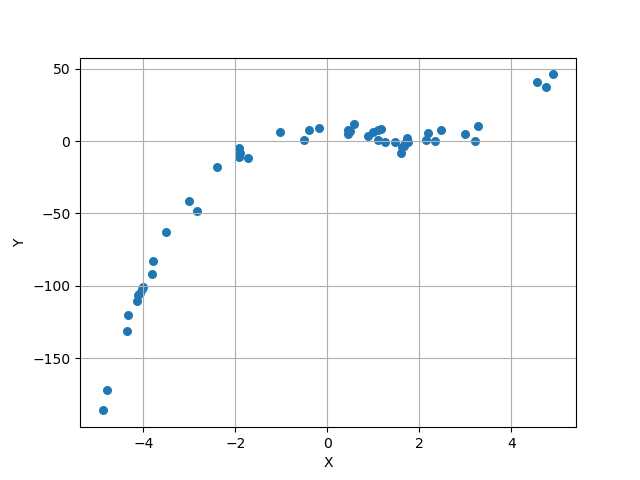
\includegraphics[width=0.5\hsize]{sq_in.png}
        \caption{近似する点列}\label{fig:sq_ingraph}            
    \end{center}
\end{figure}

\subsection{最小二乗法}
最小二乗法は、誤差を最小化するための考え方の一つである。
最小二乗法において、誤差を以下で定義する。
ラグランジュ補間の項同様に、\(n\)は入力として与えられる点の数、
\((x_i,y_i)\)は、その座標である。
\begin{equation}
    j=\sum^{n-1}_{i=0} ( f(x_i)-y_{i} )^2
    \label{eq:sq}
\end{equation}

ここで、\(f(x)\)をm個の関数\(g_k(x)\)の線形結合とおくと、
\begin{equation}
    f(x)=\sum^{m-1}_{k=0}a_{k}g_k(x)
\end{equation}
ここで式\ref{eq:sq}をみる。与えられた\((x_i,y_i)\)を定数と考える。

\(f(x_i)\)は\(x_i\)が定数であることから、
\(a_k\)の関数であるとみることができる。\(y_i\)は定数なので、
式\ref{eq:sq}は\(a_k\)の関数である。
\[
    j(a_0,a_1,\ldots,a_{n-1})=\sum^{n-1}_{i=0} ( f(x_i)-y_{i} )^2
\]

さて、そうなると、\(\exists a_k\)で、jを最小にすることができる。
jは誤差の大きさであるから、jの最小を求めることで、最も誤差の少ない近似
をすることができる。
jが最小値をとる条件は、次のように考える。

\(f(x)\)が\(a_k\)の一次関数の和であるから\(a_k\)の
一次関数である。

\(j\)は\(f(x)\)の2乗の和からなっていて、その2乗の符号は正であることから、
\(a_k\)の下に凸の二次関数である。よって、その微分が0になる点で唯一の極小値を
とってそれが最小値となる。だから、

\begin{equation}
    \frac{\partial }{\partial a_k}j(a_0,a_1,\ldots,a_{n-1})
    \label{eq:minimize}
\end{equation}

がすべての\(k=0,1,\cdots m-1\)で0になるとき、\(j\)は最小になる。
\subsection{計算手法}
前項で示された式\ref{eq:minimize}は、微分を含み、そのままでは計算しにくい。そこで、行列などを
用いて、計算しやすい形を求める。

式\ref{eq:minimize}に式\ref{eq:sq}を代入して
\begin{equation}
    \frac{\partial }{\partial a_k}\sum^{n-1}_{i=0} ( f(x_i)-y_{i} )^2
\end{equation}
これを全ての\(k\)について0にするのだった。足し合わされている項
それぞれに微分を適用して、
\begin{equation}
    \sum^{n-1}_{i=0}( f(x_i)-y_i ) \frac{\partial }{\partial a_k}( f(x_i)-y_i )
\end{equation}

ここで、
\begin{eqnarray}
    &&\frac{\partial }{\partial a_k}( f(x_i)-y_i )\label{eq:seirimael}\nonumber \\ &=&
    \frac{\partial }{\partial a_k}(\sum^{m-1}_{j=0} a_j g_j(x) - y_i )\nonumber\\ &=&
    \frac{\partial }{\partial a_k}g_k(x_i)\label{eq:seirimaer}
\end{eqnarray}
である。(\(j\neq k\)の場合、\(a_jg_j(x)\)は\(a_k\)に対して
一定なので、微分が0になることに注意。もちろん\(y_i\)は\(a_k\)に対して
一定である。)

ここで、式\ref{eq:seirimael}を行列の形に整理すると、左辺は、

\begin{eqnarray*}
    &&
    \sum^{n-1}_{i=0}
    \left(
      \begin{array}{cccc}
        g_0(x_i)g_k(x_i) & g_1(x_i)g_k(x_i) & \cdots & g_{m-1}(x_i)g_k(x_i)
      \end{array}
    \right)
    \left(
      \begin{array}{c}
        a_0 \\ a_1 \\ \vdots \\ a_{m-1}
      \end{array}
    \right)
    \\ &=&
    \left(
      \begin{array}{cccc}
        g_k(x_0) & g_k(x_1) & \cdots & g_k(x_{n-1})
      \end{array}
    \right)
    \left(
      \begin{array}{cccc}
        g_0(x_0) & g_1(x_0) & \cdots & g_{m-1}(x_0) \\
        g_0(x_1) & g_1(x_1) & \cdots & g_{m-1}(x_0) \\
        \vdots & \vdots & \ddots & \vdots \\
        g_0(x_{n-1}) & g_1(x_{n-1}) & \cdots & g_{m-1}(x_{n-1})  
      \end{array}
    \right)
    \left(
      \begin{array}{c}
        a_0 \\ a_1 \\ \vdots \\ a_{m-1}
      \end{array}
    \right)
\end{eqnarray*}
式\ref{eq:seirimaer}は、
\begin{eqnarray*}
    \left(
      \begin{array}{cccc}
        g_k(x_0) & g_k(x_1) & \cdots & g_k(x_{n-1})
      \end{array}
    \right)
    \left(
      \begin{array}{c}
        y_0 \\ y_1 \\ \vdots \\ y_{n-1}
      \end{array}
    \right)
\end{eqnarray*}
すべてのkについて縦に積み重ねて、一つの式にすると、
\begin{eqnarray}
    \left(
      \begin{array}{cccc}
        g_0(x_0) & g_0(x_1) & \cdots & g_0(x_{n-1}) \\
        g_1(x_0) & g_1(x_1) & \cdots & g_1(x_{n-1}) \\
        \vdots & \vdots & \ddots & \vdots \\
        g_{m-1}(x_0) & g_{m-1}(x_1) & \cdots & g_{m-1}(x_{n-1}) \\
      \end{array}
    \right)
    \left(
      \begin{array}{cccc}
        g_0(x_0) & g_1(x_0) & \cdots & g_{m-1}(x_0) \\
        g_0(x_1) & g_1(x_1) & \cdots & g_{m-1}(x_0) \\
        \vdots & \vdots & \ddots & \vdots \\
        g_0(x_{n-1}) & g_1(x_{n-1}) & \cdots & g_{m-1}(x_{n-1})  
      \end{array}
    \right)
    \left(
      \begin{array}{c}
        a_0 \\ a_1 \\ \vdots \\ a_{m-1}
      \end{array}
    \right)\nonumber \\
    =\left(
        \begin{array}{cccc}
          g_0(x_0) & g_0(x_1) & \cdots & g_0(x_{n-1}) \\
          g_1(x_0) & g_1(x_1) & \cdots & g_1(x_{n-1}) \\
          \vdots & \vdots & \ddots & \vdots \\
          g_{m-1}(x_0) &  g_{m-1}(x_1) & \cdots &  g_{m-1}(x_{n-1}) \\
        \end{array}
      \right)
    \left(
      \begin{array}{c}
        y_0 \\ y_1 \\ \vdots \\ y_{n-1}
      \end{array}
    \right)
\end{eqnarray}
が成り立つことがわかる。
以下のように\(G,a,y\)をおくと、
\begin{eqnarray*}
    G&=&
    \left(
      \begin{array}{cccc}
        g_0(x_0) & g_1(x_0) & \cdots & g_{m-1}(x_0) \\
        g_0(x_1) & g_1(x_1) & \cdots & g_{m-1}(x_0) \\
        \vdots & \vdots & \ddots & \vdots \\
        g_0(x_{n-1}) & g_1(x_{n-1}) & \cdots & g_{m-1}(x_{n-1})  
      \end{array}
    \right)\\
    a&=&
    \left(
        \begin{array}{c}
            a_0 \\ a_1 \\ \vdots \\ g_{m-1}
        \end{array}
    \right)\\
    y&=&
    \left(
        \begin{array}{c}
            y_0 \\ y_1 \\ \vdots \\ y_{n-1}
        \end{array}
    \right)
\end{eqnarray*}
以下のように書ける。
\begin{eqnarray*}
    G^\mathrm{T}Ga&=&G^\mathrm{T}y\\
    a&=&(G^\mathrm{T}G)^{-1}G^\mathrm{T}y\label{eq:sqeqlast}
\end{eqnarray*}
さて、\(f(x)\)はm個の関数\(g_k(x)\)の線形結合であった。
例えば、\(x^n\)(nは整数)の線形結合でできた
多項式による近似を考えると、行列\(G\)は
以下のようになる。
\[
    G=\left(
        \begin{array}{cccc}
          g_0(x_0) & g_1(x_0) & \cdots & g_{m-1}(x_0) \\
          g_0(x_1) & g_1(x_1) & \cdots & g_{m-1}(x_0) \\
          \vdots & \vdots & \ddots & \vdots \\
          g_0(x_{n-1}) & g_1(x_{n-1}) & \cdots & g_{m-1}(x_{n-1})  
        \end{array}
      \right)=
    \left(
      \begin{array}{cccc}
        1 & x_0^1 & \cdots & x_0^{m-1} \\
        1 & x_1^1 & \cdots & x_1^{m-1} \\
        \vdots & \vdots & \ddots & \vdots \\
        1 & x_{n-1}^1 & \cdots & x_{n-1}^{m-1} 
      \end{array}
    \right)
\]
これで、計算をするための式が求められた。
\subsection{結果と考察}
まず、図\ref{fig:lag_ingraph} に表される点列をn-1次関数で近似し(nは1から5までの整数)
どれだけ正確に点列を近似できているか調べる。
近似する点と、得られた関数を次の図に示す。
\begin{figure}[htbp]
    \begin{center}
        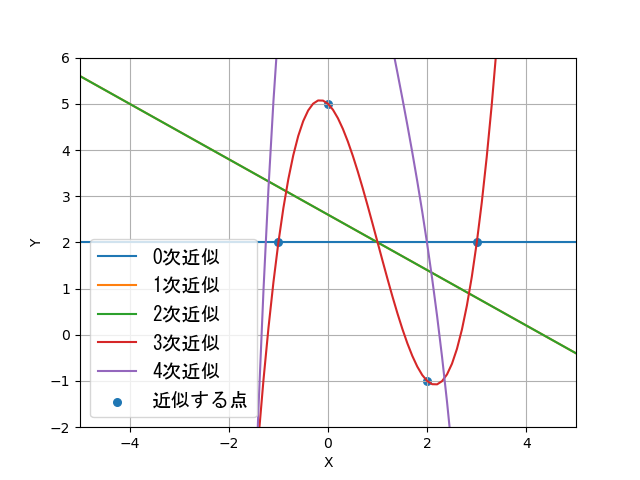
\includegraphics[width=0.5\hsize]{sq_ex1.png}
        \caption{4点の最小二乗法による近似}\label{fig:sq_ex1}           
    \end{center}
\end{figure}
前述したが、この4点を通る3次関数は、\(y=x^3-3x^2-x+5\)である。

それぞれ求められた式は、以下である。ただし、実際の出力を
小数点第3位で四捨五入した。
\begin{eqnarray*}
    y&=&2.00\\
    y&=&-0.6x+2.60\\
    y&=&0.00x^2-0.60x+2.60\\
    y&=&1.00x^3-3.00x^2-1.00x+5.00\\
    y&=&-0.46x^4+2.09x^3-4.00x^2-1.53x+11.68
\end{eqnarray*}
3次の近似式は、ほとんど完全に与えた4点を通る3次関数と一致した。
一方、4次の近似式は、説明のつかないような値になっている。
これは、式\ref{eq:sqeqlast}における\(G^\mathrm{T}G\)が逆行列
を持たないために、計算が破綻したからだと考えられる。
一般に、\(n\times m\)行列とその転置行列の積は\(n \times m\)行列
になるが、\(m>n\)の場合、その逆行列は存在しない。今回の場合は、与えられた点の
数が\(n\)、近似する次数が\(m-1\)であるから、4つの点を4次関数で近似
しようとすると、\(G\)の逆行列が存在しなくなる。

次に、図\ref{fig:sq_ingraph}に表される点列をn-1次関数で近似し(nは1から5までの整数)
どれだけ正確に点列を近似できているか調べる。
近似する点と、得られた関数を次の図に示す。
\begin{figure}[htbp]
    \begin{center}
        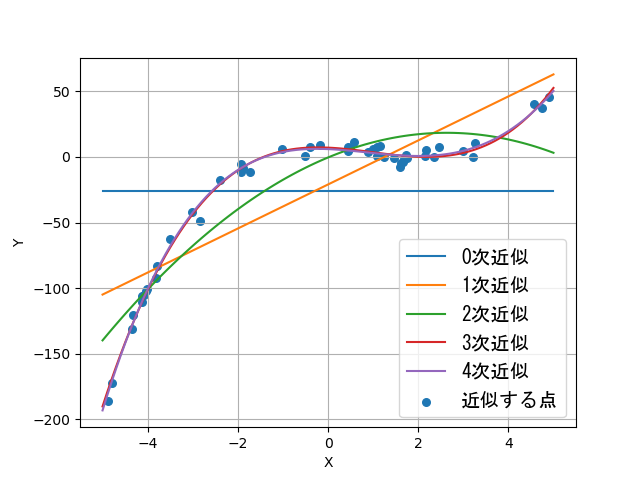
\includegraphics[width=0.5\hsize]{sq_ex2.png}
        \caption{点列の最小二乗法による近似}\label{fig:sq_ex2}            
    \end{center}
\end{figure}
それぞれ求められた式は、以下である。
\begin{eqnarray*}
    y&=& -26.02\\
    y&=& 16.78x-20.10\\
    y&=& -2.72x^2-14.29x-0.42\\
    y&=& 1.03x^3-3.03x^2-1.52x+7.08\\
    y&=&-0.02x^4+1.03x^3-2.56x^2-1.44x+5.96
\end{eqnarray*}
図をみる通り、近似の次数が上がるとより点の並びに近い関数になっていることがわかる。
\newpage
\appendix
\section{\(m>n\)で\(G^\mathrm{T}G\)の逆行列が存在しないことの証明}
\(A\)を\(n\times m\)行列とする。ただし、\(m>n\)とする。これは、行列\(G\)を
含む形になっている。

\(A\)の要素を次のように書く。
\begin{equation}
    A=
    \left(
    \begin{array}{cccc}
        A_{0,0} & A_{0,1} & \cdots & A_{0,m-1} \\
        A_{1,0} & A_{1,1} & \cdots & A_{1,m-1} \\
        \vdots & \vdots & \ddots & \vdots \\
        A_{n-1,0} &A_{n-1,1} & \cdots & A_{n-1,m-1}
    \end{array}
    \right)
\end{equation}

\(A\)の行列式が\(0\)になることを示す。

\(A^\mathrm{T}A\)の行列式は次のように書ける。
\begin{equation}
    |A^\mathrm{T}A|=
    \left|
    \begin{array}{cccc}
        \sum^{n-1}_{k=0}A_{k,0}A_{k,0} & \sum^{n-1}_{k=0}A_{k,0}A_{k,1} & \cdots & \sum^{n-1}_{k=0}A_{k,0}A_{k,m-1} \\
        \sum^{n-1}_{k=0}A_{k,1}A_{k,0} & \sum^{n-1}_{k=0}A_{k,1}A_{k,1} & \cdots & \sum^{n-1}_{k=0}A_{k,1}A_{k,m-1} \\
        \vdots & \vdots & \ddots & \vdots \\
        \sum^{n-1}_{k=0}A_{k,m-1}A_{k,0} &\sum^{n-1}_{k=0}A_{k,m-1}A_{k,1} & \cdots & \sum^{n-1}_{k=0}A_{k,m-1}A_{k,m-1}
    \end{array}
    \right|
\end{equation}
行列式の和の性質を使い、1行目について分離すると、
\begin{eqnarray*}
    |A^\mathrm{T}A|&=&
    \sum^{n-1}_{k_0=0}
    \left|
    \begin{array}{cccc}
        A_{k_0,0}A_{k_0,0} & A_{k_0,0}A_{k_0,1} & \cdots & A_{k_0,0}A_{k_0,m-1} \\
        \sum^{n-1}_{k=0}A_{k,1}A_{k,0} & \sum^{n-1}_{k=0}A_{k,1}A_{k,1} & \cdots & \sum^{n-1}_{k=0}A_{k,1}A_{k,m-1} \\
        \vdots & \vdots & \ddots & \vdots \\
        \sum^{n-1}_{k=0}A_{k,m-1}A_{k,0} &\sum^{n-1}_{k=0}A_{k,m-1}A_{k,1} & \cdots & \sum^{n-1}_{k=0}A_{k,m-1}A_{k,m-1}
    \end{array}
    \right|\\
    &=&
    \sum^{n-1}_{k_0=0}A_{k_0,0}
    \left|
    \begin{array}{cccc}
        A_{k_0,0} & A_{k_0,1} & \cdots & A_{k_0,m-1} \\
        \sum^{n-1}_{k=0}A_{1,k}A_{0,k} & \sum^{n-1}_{k=0}A_{1,k}A_{1,k} & \cdots & \sum^{n-1}_{k=0}A_{1,k}A_{n-1,k} \\
        \vdots & \vdots & \ddots & \vdots \\
        \sum^{n-1}_{k=0}A_{n-1,k}A_{0,k} &\sum^{n-1}_{k=0}A_{n-1,k}A_{1,k} & \cdots & \sum^{n-1}_{k=0}A_{n-1,k}A_{n-1,k}
    \end{array}
    \right|
\end{eqnarray*}
同様に第2~第n-1行について分離すると、
\begin{eqnarray}
    |A^\mathrm{T}A|&=&
    \sum^{n-1}_{k_0=0}A_{k_0,0}
    \sum^{n-1}_{k_1=0}A_{k_1,0}
    \left|
    \begin{array}{cccc}
        A_{k_0,0} & A_{k_0,1} & \cdots & A_{k_0,m-1} \\
        A_{k_1,0} & A_{k_1,1} & \cdots & A_{k_1,m-1} \\
        \vdots & \vdots & \ddots & \vdots \\
        \sum^{n-1}_{k=0}A_{n-1,k}A_{0,k} &\sum^{n-1}_{k=0}A_{n-1,k}A_{1,k} & \cdots & \sum^{n-1}_{k=0}A_{n-1,k}A_{n-1,k}
    \end{array}
    \right|\\
    &=&
    \prod^{m-1}_{l=0}
    \sum^{n-1}_{k_l=0}A_{0,k_l}
    \left|
    \begin{array}{cccc}
        A_{k_0,0} & A_{k_0,1} & \cdots & A_{k_0,m-1} \\
        A_{k_1,0} & A_{k_1,1} & \cdots & A_{k_1,m-1} \\
        \vdots & \vdots & \ddots & \vdots \\
        A_{k_{m-1},0} & A_{k_{m-1},1} & \cdots & A_{k_{m-1},m-1} \\
    \end{array}
    \right|\label{eq:gyouretusiki}
\end{eqnarray}

式\ref{eq:gyouretusiki}の行列式内の数値は、

行列に同じ行が2つあると行列式が0になる

という性質より、\(k_0,k_1,\ldots,k_{m-1}\)がすべて異なる値の場合のみ0でない。
しかし、\(k\)は整数であり、\(0\)から\(n-1\)までの\(n\)通りの値しかとることができない。
\(m>n\)のとき、鳩の巣原理より必ず\(k_0,k_1,\ldots,k_{m-1}\)のいずれかの組が同じ値に
なり、行列式は0となる。なので、全体の行列式も0になる。


\end{document}